\footnotesize
\begin{multicols}{2}[\columnsep=0.4cm]
    Methanogenic activity requires lab enrichment and methanogenic activity validation, therefore putative methanogens and methanotrophs are addressed as MCR-encoding MAGs.

    \vspace{0.2cm}
    
    MCR-encoding MAGs are found in the NSPSF dataset, belonging to taxonomic groups c\_\_Bog-38 (class Bog-38, according to GTDB release 220) \cite{Chaumeil_2022_gtdbtk}, f\_\_JACTUA01, g\_\_ANME-1-THS, g\_\_Methanobacterium\_A and f\_\_JACAEJ01. Bog-38 demonstrated the highest abundance amongst MCR-encoding MAGs, as well being highly prevalent across different sites, although mostly absent at the surface.

    \begin{figure}[H]
        \vspace{-0.4cm}
        \centering
        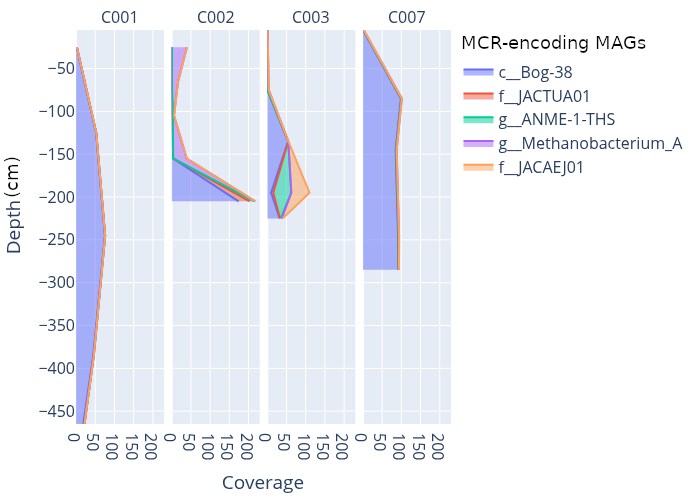
\includegraphics[width=\linewidth]{content-images/abundance_depth.png}
        \caption{\scriptsize Coverage of MCR-encoding archaeal groups across sampling sites and depths. Coverage refers to the average sequencing depth of each MAG, calculated as the mean number of reads mapped per base pair of the genome, providing an estimate of its relative abundance in the sample.}
        \label{fig:coverage}
    \end{figure}  

    \vspace{-0.4cm}
    
    We constructed a Bog-38 maximum likelihood phylogenomic tree from concatenation of 76 single-copy core genes, consisting of MAGs from the NSPSF dataset as well as from the Genome Taxonomy Database (GTDB) release 220 (Figure \ref{fig:phylo}) \cite{Lee_2019_gtotree}. Inclusion of NSPSF MAGs contributed immensely in phylogenetic gain of Bog-38 by 73.4\%. Several NSPSF MAGs form unique clades, where these MAGs cluster away from GTDB MAGs. Almost 90\% of these GTDB MAGs originate from shotgun metagenomic projects of the Stordalen Mire in Sweden, and are taxonomically associated to \emph{Methanoflorens stordalenmirensis} \cite{Mondav_2014_Methanoflorens} and \emph{Methanoflorens crillii} \cite{Woodcroft_2018_permafrost}. The earliest reported genome from the genus \emph{Methanoflorens} (referred as g\_\_Bog-38 in GTDB) was reported in 2014 \cite{Mondav_2014_Methanoflorens}. According to GTDB, \textit{Methanoflorens} is the only genus currently assigned to the class c\_\_Bog-38. Further work will be used to confirm taxonomic placement of these new class Bog-38 MAGs from NSPSF and if they possess unique biochemistry compared to the two \emph{Methanoflorens} species.

    Genomic annotation of high-quality Bog-38 MAGs confirmed putative hydrogenotrophic methanogenesis activity, as suggested previously with \textit{Methanoflorens stordalenmirensis} \cite{Mondav_2014_Methanoflorens}. Further inspection also reveals putative nitrogen fixation activity, as revealed by the presence of \textit{nifHDK} gene cluster.
    
    \begin{figure}[H]
        \vspace{-0.4cm}
        \centering
        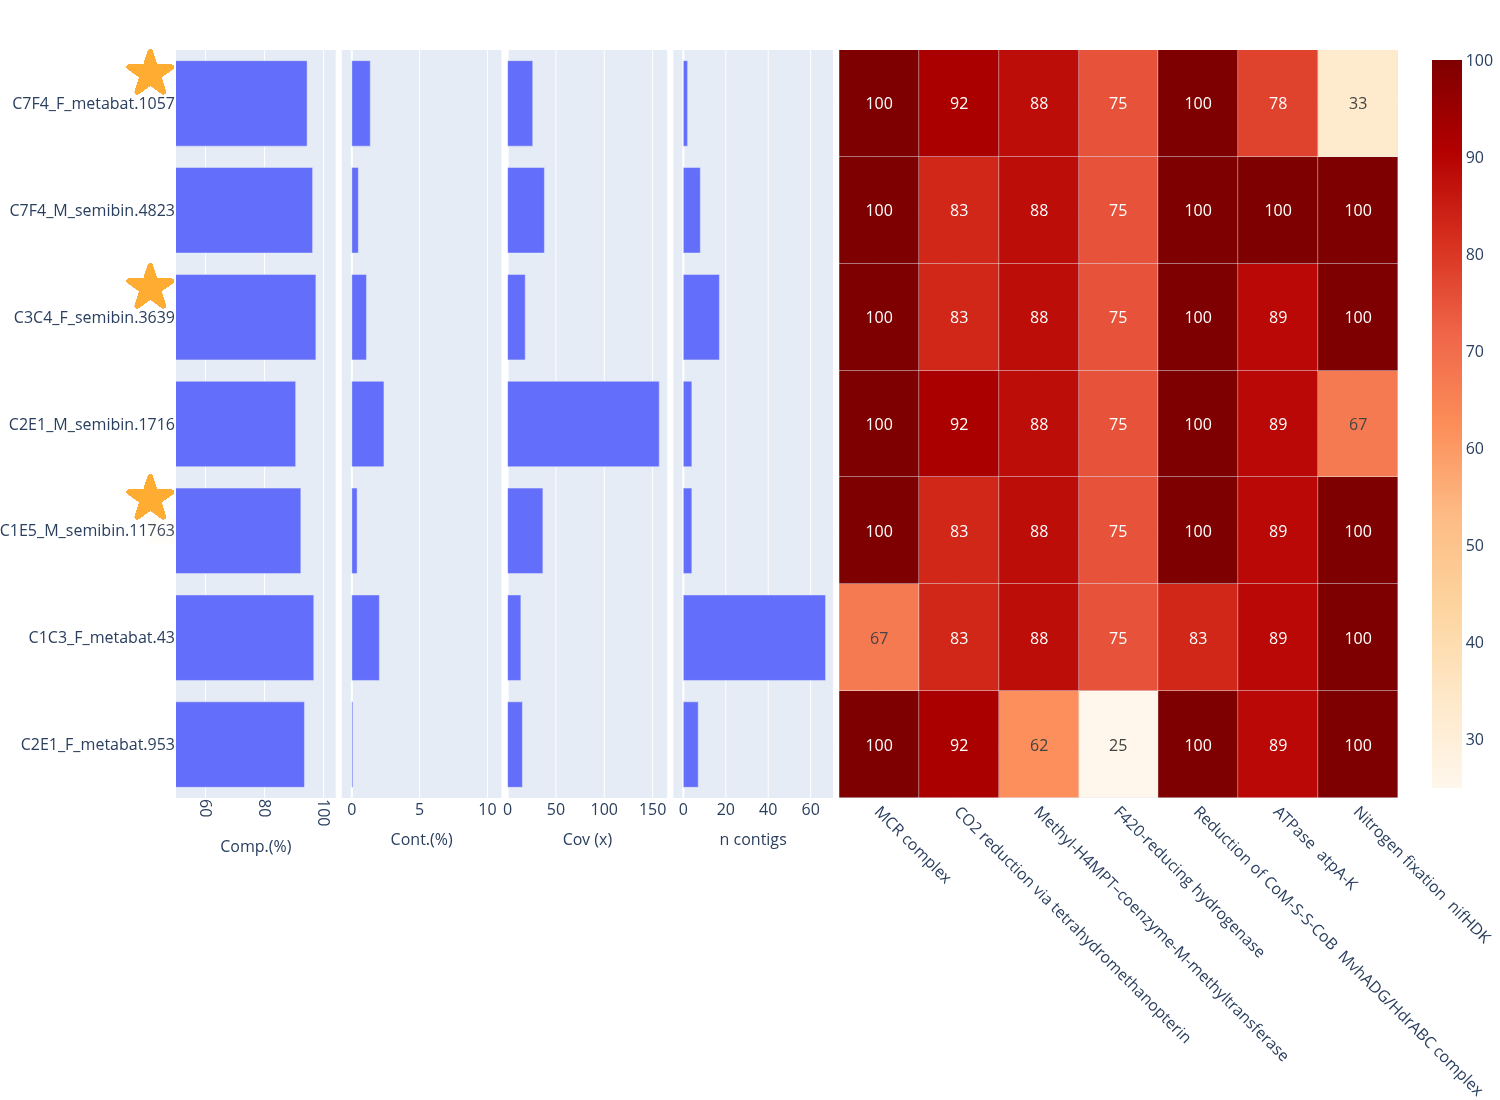
\includegraphics[width=\linewidth]{content-images/heatmap.png}
        \caption{\scriptsize CH$_4$ metabolism genes encoded by MCR-containing MAGs. MAG ID labels are shown on the left; only high-quality MAGs are included (minimum 90\% completeness, maximum 5\% contamination). Bar plots to the left of the heatmaps show MAG completeness, contamination, average read coverage per sample, and the number of contigs. Heatmap colors and values represent the completeness of each genetic component as a percentage. Genomes that we successfully assembled to singular circular contigs are annotated with stars.}
        \label{fig:heatmap}
    \end{figure}

    \vspace{-0.4cm}
    Three MAGs were further curated and successfully yield complete singular circular chromosome \ref{fig:heatmap}. The successful recovery of complete genomes of Bog-38 from NSPSF further proves their presence in the environment. This finding contrasts with their absence in another tropical peat soil environment, the Maludam National Park in Sarawak. 
    
    % \vspace{1.5em}

    % \begin{tcolorbox}
    % \lipsum[66]
    % \end{tcolorbox}
\end{multicols}

% \vspace{1.5em} % spacing before the full-width figure

% ---- Full-width TikZ block (outside multicols) ----
\begin{figure}[H]
    \vspace{-0.4cm}
    \centering
    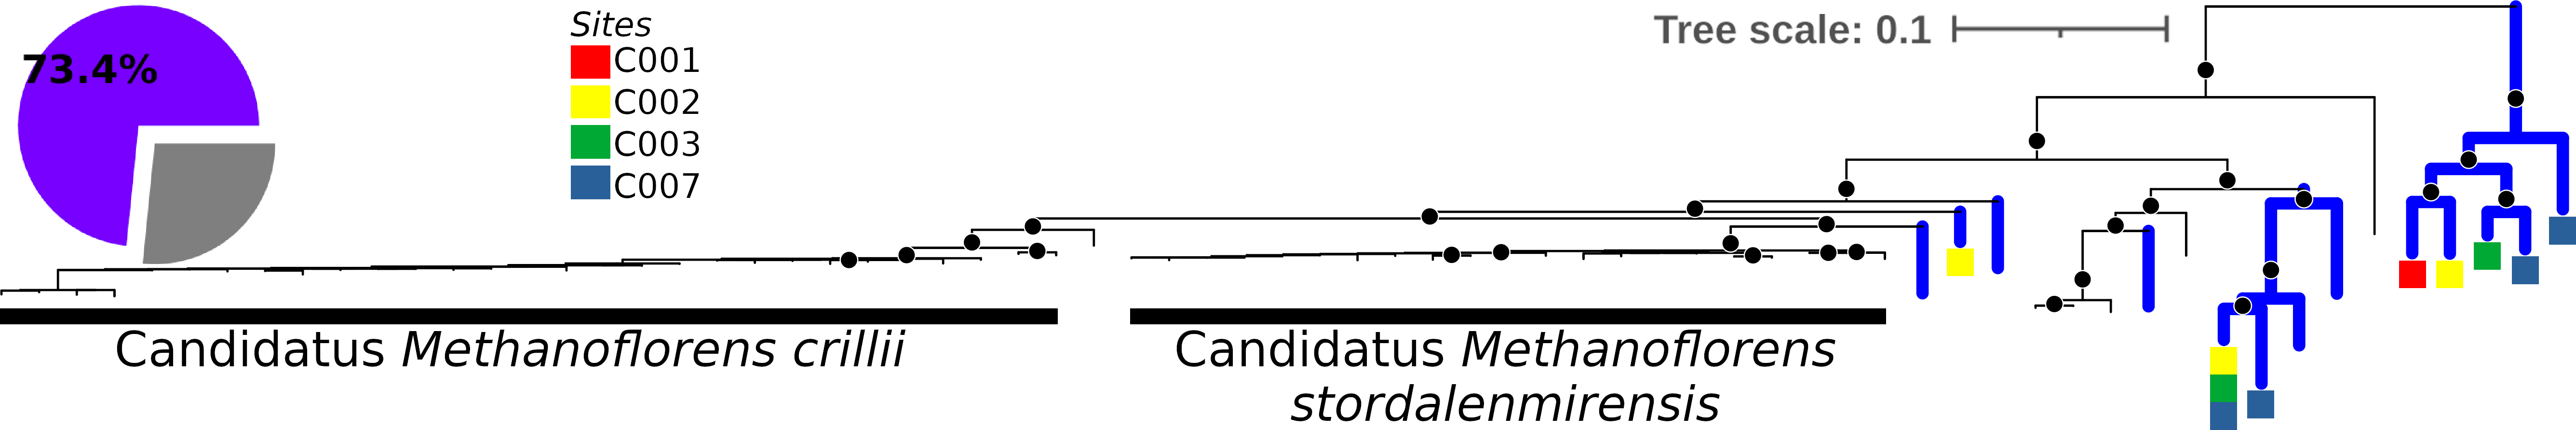
\includegraphics[width=\linewidth]{content-images/bog38_invert.png}
    \caption{\scriptsize Phylogenomic tree of archaeal class Bog-38. Candidatus \emph{Methanoflorens stordalenmirensis} and Candidatus \emph{Methanoflorens crillii} are indicated. Colored branches indicate MAGs that originate from the NSPSF dataset. Pie charts indicate increase in phylogenetic diversity from inclusion of NSPSF MAGs relative to currently available genomes in the public database (last accessed \nth{15} January 2025). Phylogenomic trees were rooted using outgroup c\_\_Methanomicrobia, which were removed from the final visualization. Bootstrap supports are indicated by black dots ranging from 90-100\%. Tree scale is 0.1. A MAG is deemed as present in a site if average coverage values are at least 10 in a site.}
    \label{fig:phylo}
\end{figure}  